% Options for packages loaded elsewhere
\PassOptionsToPackage{unicode}{hyperref}
\PassOptionsToPackage{hyphens}{url}
%
\documentclass[
]{article}
\usepackage{amsmath,amssymb}
\usepackage{iftex}
\ifPDFTeX
  \usepackage[T1]{fontenc}
  \usepackage[utf8]{inputenc}
  \usepackage{textcomp} % provide euro and other symbols
\else % if luatex or xetex
  \usepackage{unicode-math} % this also loads fontspec
  \defaultfontfeatures{Scale=MatchLowercase}
  \defaultfontfeatures[\rmfamily]{Ligatures=TeX,Scale=1}
\fi
\usepackage{lmodern}
\ifPDFTeX\else
  % xetex/luatex font selection
\fi
% Use upquote if available, for straight quotes in verbatim environments
\IfFileExists{upquote.sty}{\usepackage{upquote}}{}
\IfFileExists{microtype.sty}{% use microtype if available
  \usepackage[]{microtype}
  \UseMicrotypeSet[protrusion]{basicmath} % disable protrusion for tt fonts
}{}
\makeatletter
\@ifundefined{KOMAClassName}{% if non-KOMA class
  \IfFileExists{parskip.sty}{%
    \usepackage{parskip}
  }{% else
    \setlength{\parindent}{0pt}
    \setlength{\parskip}{6pt plus 2pt minus 1pt}}
}{% if KOMA class
  \KOMAoptions{parskip=half}}
\makeatother
\usepackage{xcolor}
\usepackage[margin=1in]{geometry}
\usepackage{graphicx}
\makeatletter
\def\maxwidth{\ifdim\Gin@nat@width>\linewidth\linewidth\else\Gin@nat@width\fi}
\def\maxheight{\ifdim\Gin@nat@height>\textheight\textheight\else\Gin@nat@height\fi}
\makeatother
% Scale images if necessary, so that they will not overflow the page
% margins by default, and it is still possible to overwrite the defaults
% using explicit options in \includegraphics[width, height, ...]{}
\setkeys{Gin}{width=\maxwidth,height=\maxheight,keepaspectratio}
% Set default figure placement to htbp
\makeatletter
\def\fps@figure{htbp}
\makeatother
\setlength{\emergencystretch}{3em} % prevent overfull lines
\providecommand{\tightlist}{%
  \setlength{\itemsep}{0pt}\setlength{\parskip}{0pt}}
\setcounter{secnumdepth}{-\maxdimen} % remove section numbering
\ifLuaTeX
  \usepackage{selnolig}  % disable illegal ligatures
\fi
\IfFileExists{bookmark.sty}{\usepackage{bookmark}}{\usepackage{hyperref}}
\IfFileExists{xurl.sty}{\usepackage{xurl}}{} % add URL line breaks if available
\urlstyle{same}
\hypersetup{
  pdftitle={Wine Blind Tasting Xmas 2023},
  hidelinks,
  pdfcreator={LaTeX via pandoc}}

\title{Wine Blind Tasting Xmas 2023}
\author{}
\date{\vspace{-2.5em}}

\begin{document}
\maketitle

\hypertarget{le-bottiglie-in-gara}{%
\subsection{Le bottiglie in gara:}\label{le-bottiglie-in-gara}}

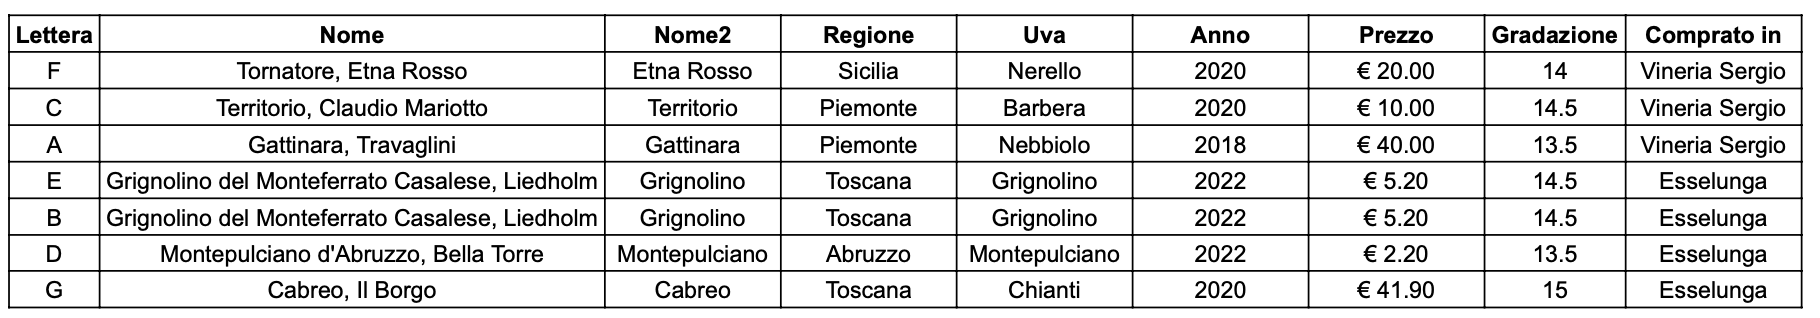
\includegraphics[width=1\linewidth]{wineinfo}

\hypertarget{indovina-la-bottiglia}{%
\subsection{Indovina la bottiglia}\label{indovina-la-bottiglia}}

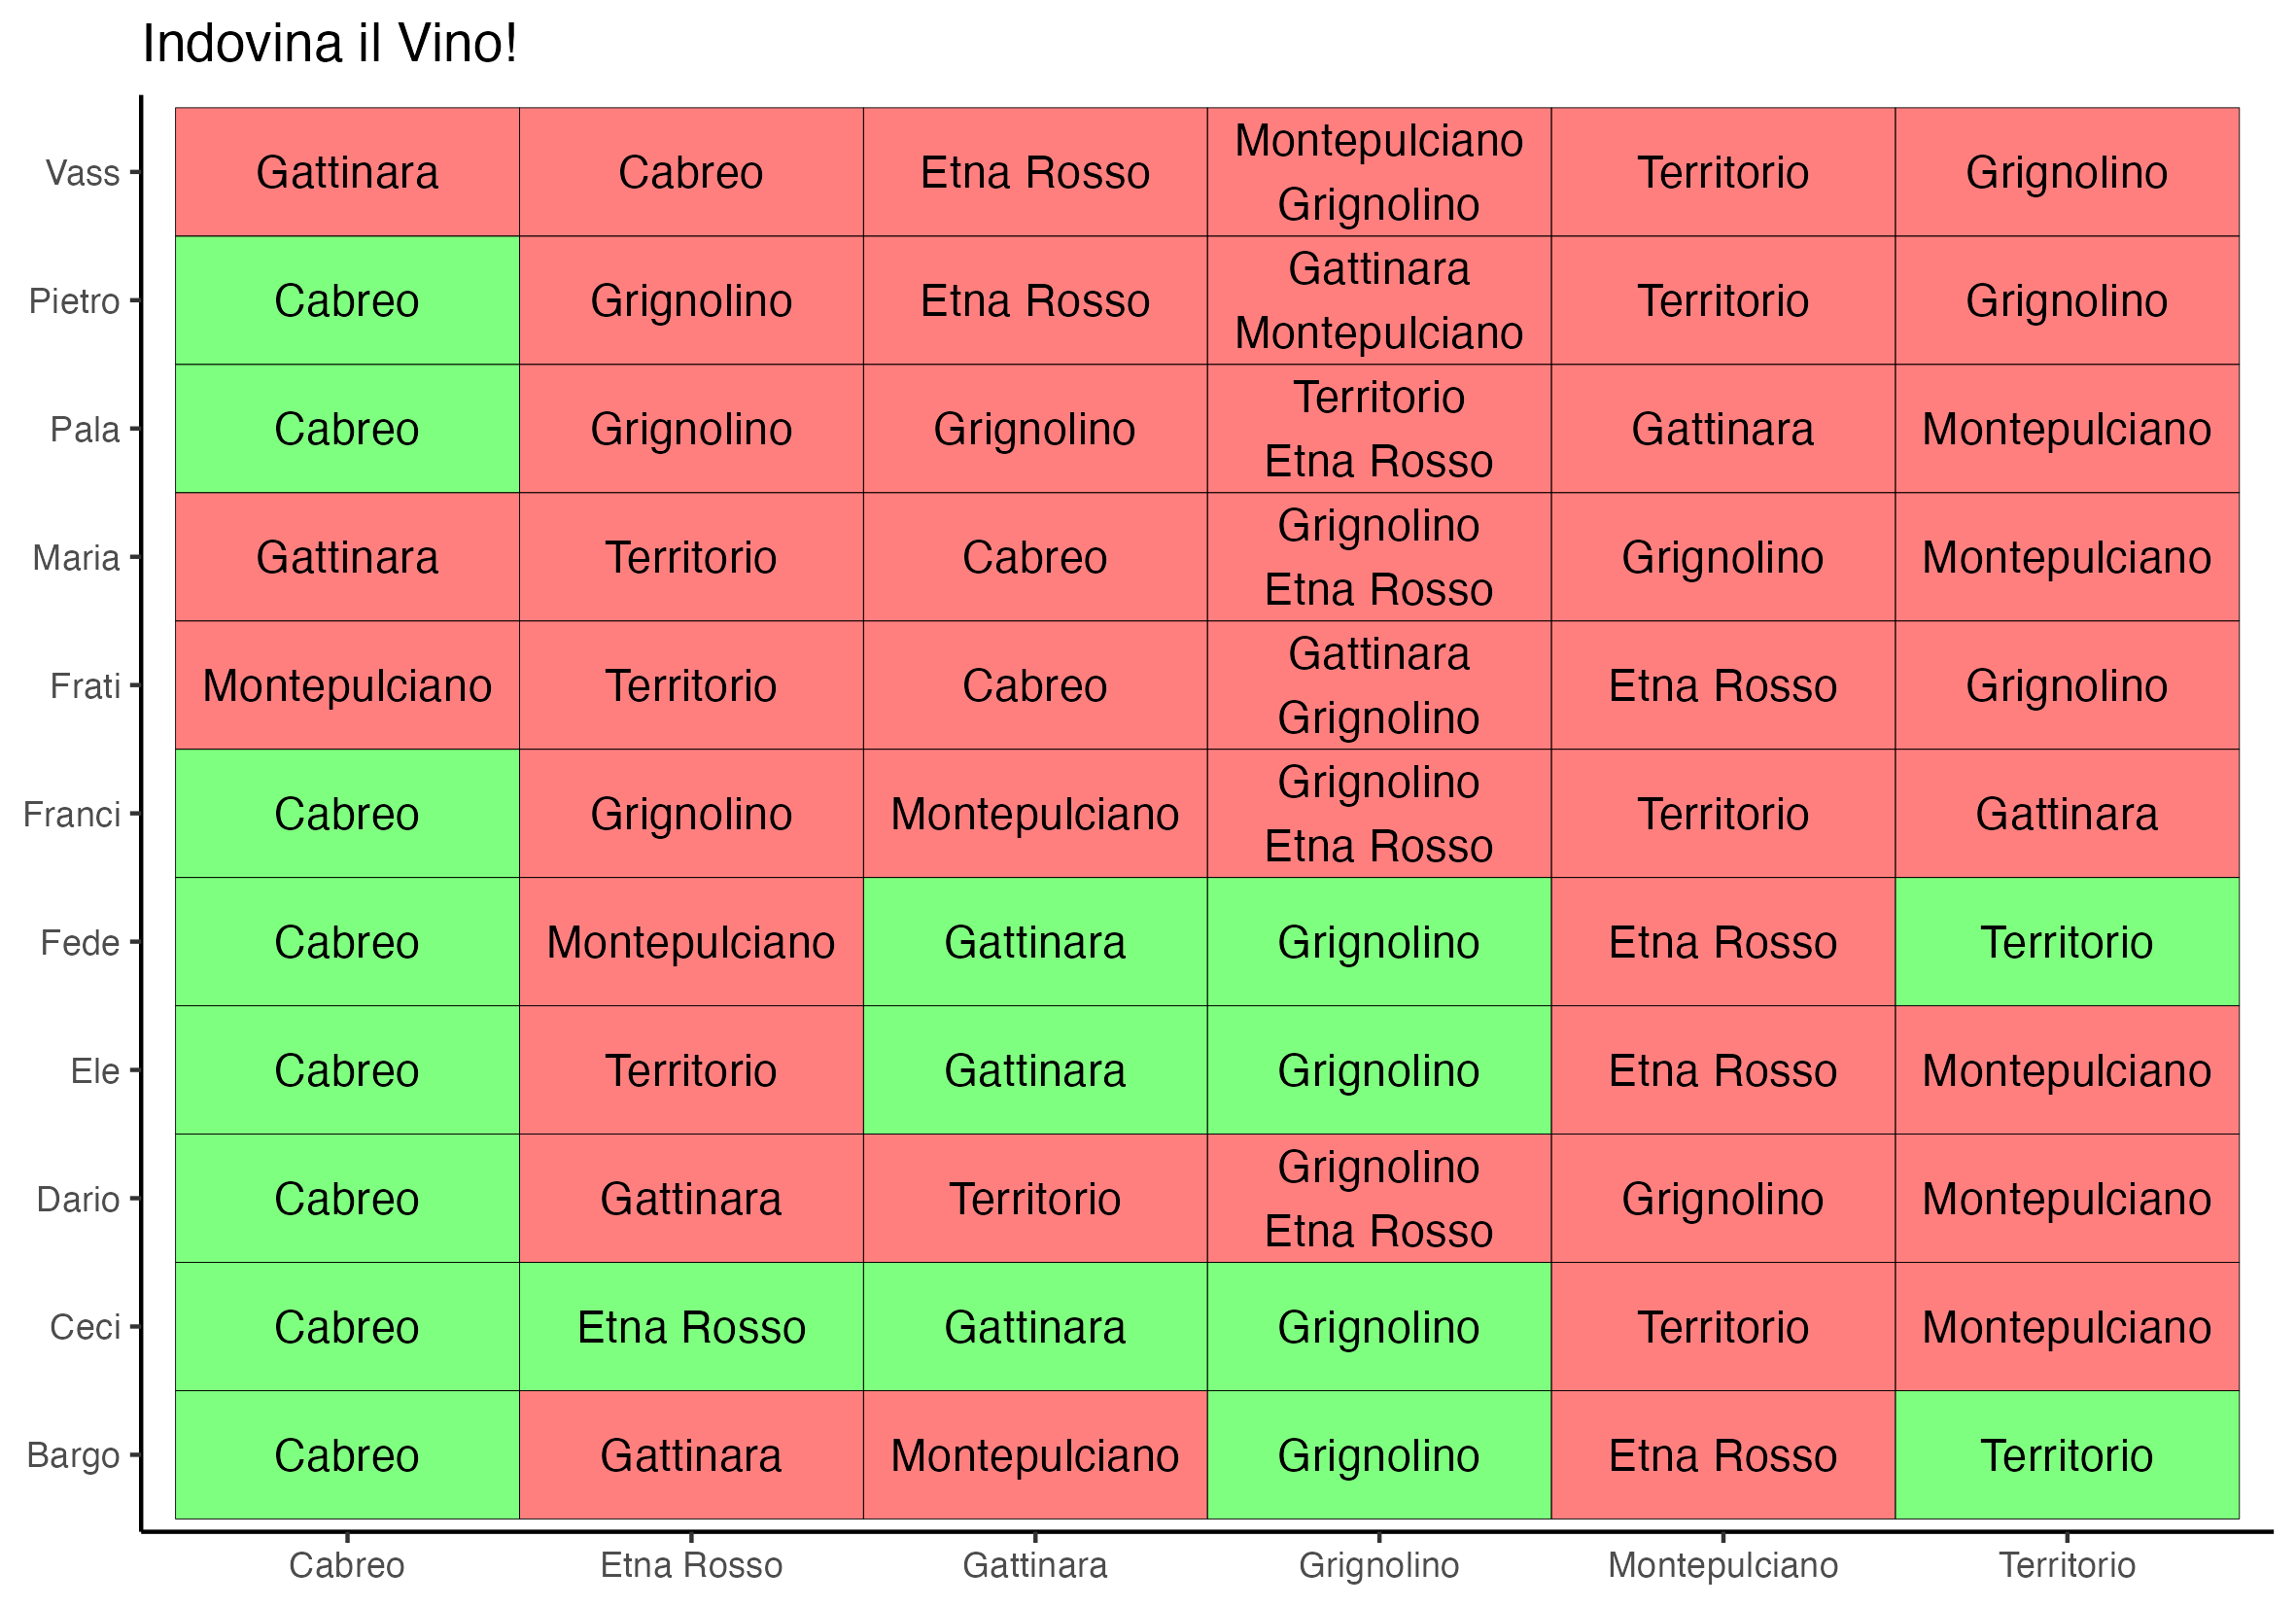
\includegraphics[width=1\linewidth]{plots/indoVino}

\hypertarget{le-bottiglie-uguali}{%
\subsection{Le bottiglie uguali}\label{le-bottiglie-uguali}}

Qualcuno non é riuscito a riconoscere le bottiglie identiche e ha
giudicato una meglio dell'altra:

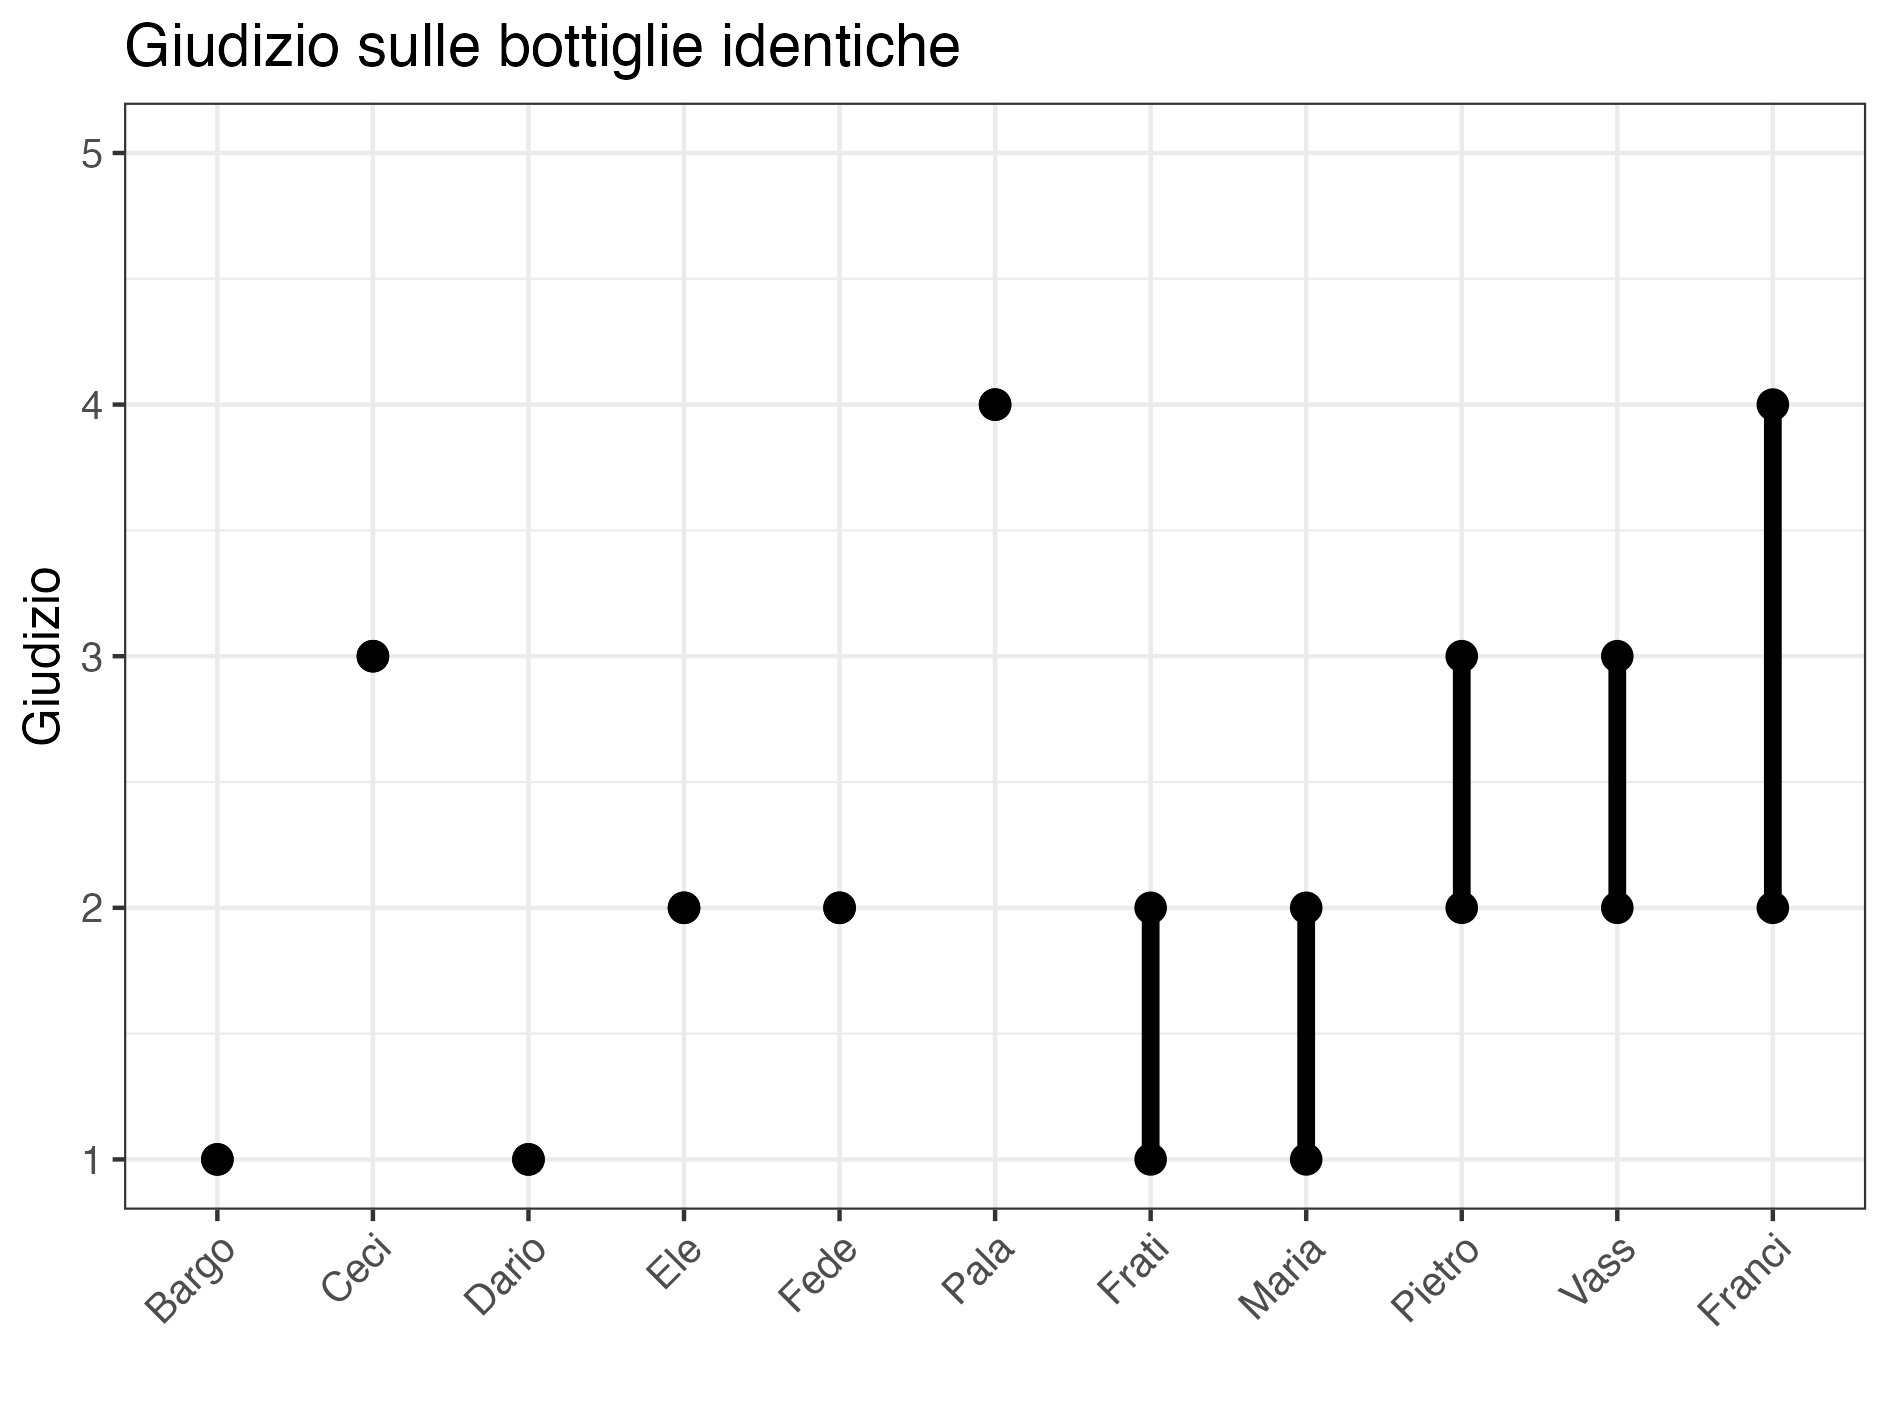
\includegraphics[width=1\linewidth]{plots/paired_wines_rating}

\hypertarget{il-miglior-vino-di-questanno}{%
\subsection{Il miglior vino di
quest'anno}\label{il-miglior-vino-di-questanno}}

Il punto rosso indica il giudizio medio.

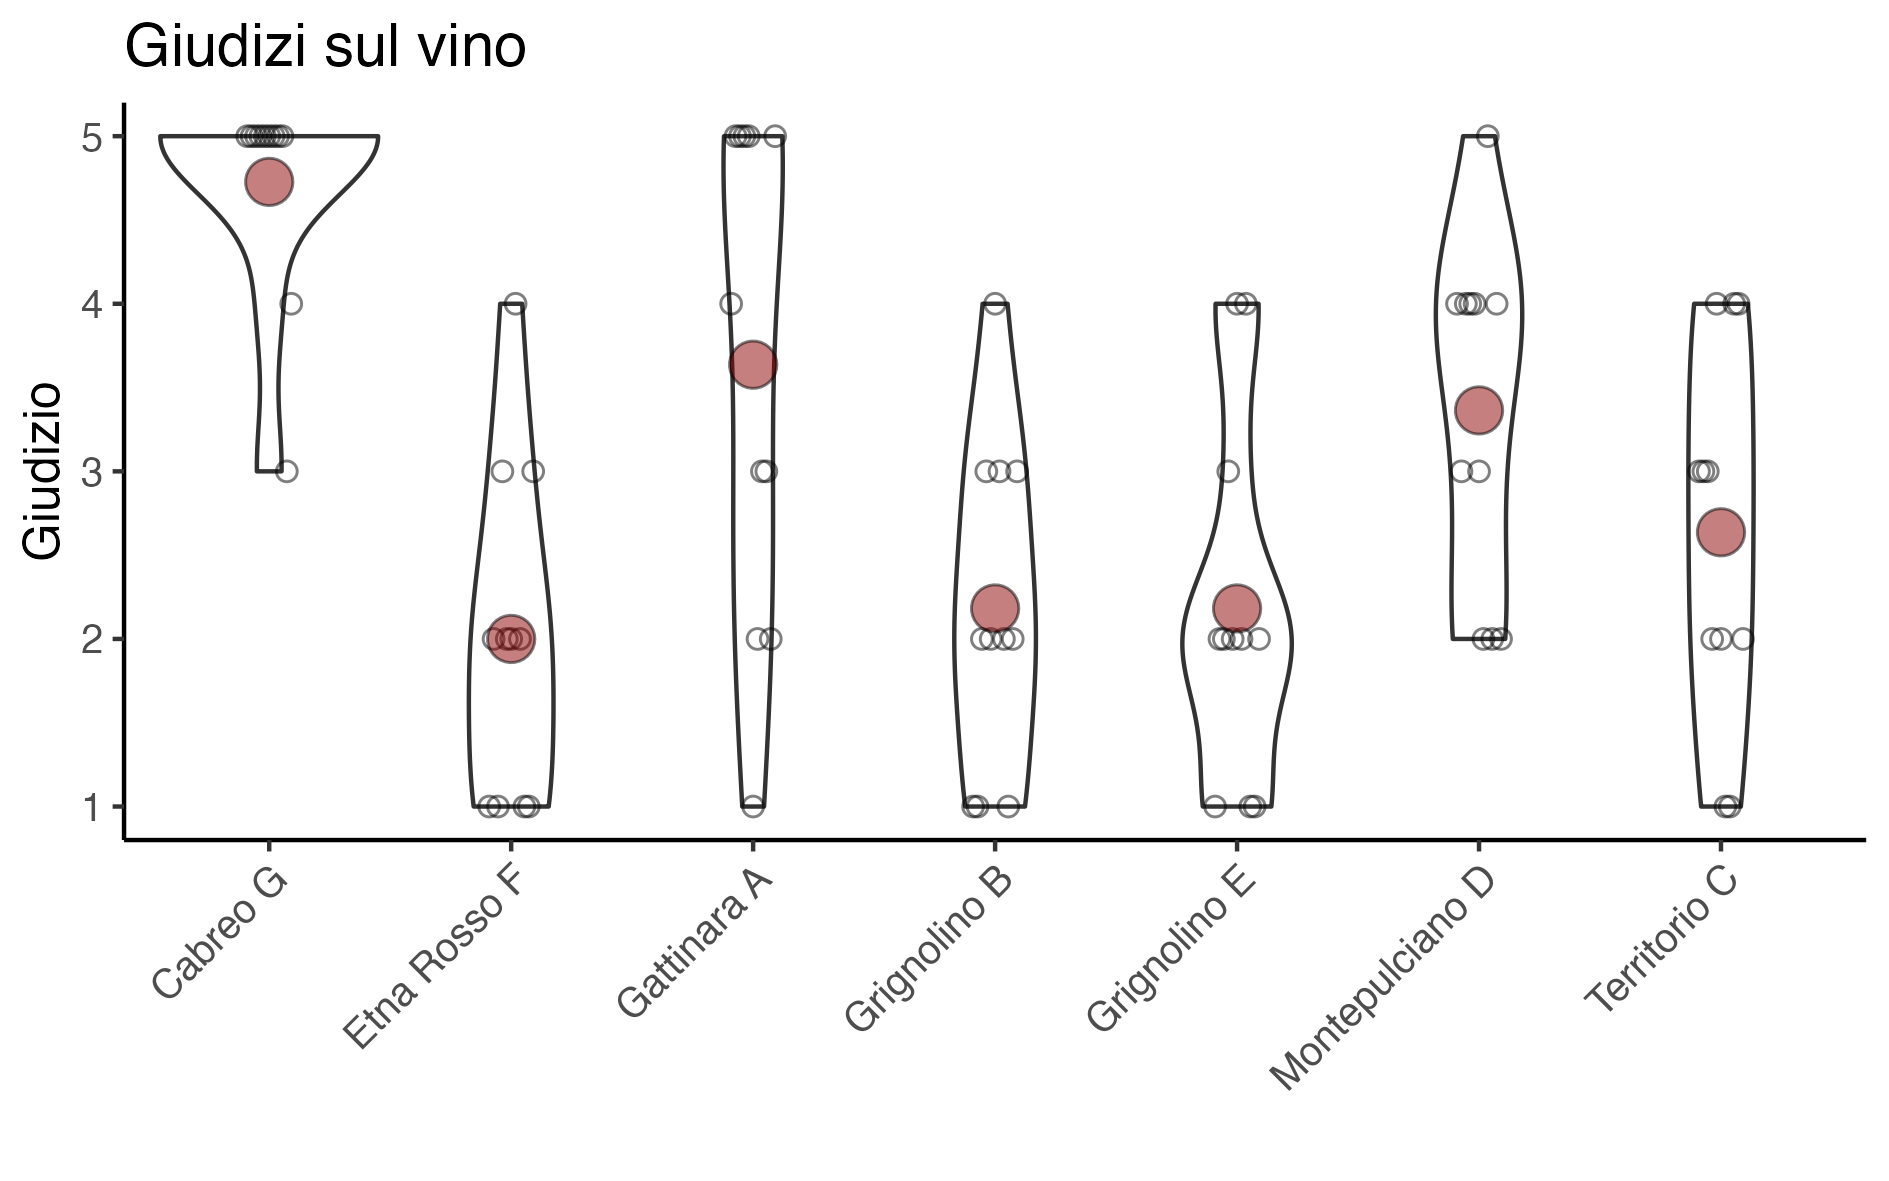
\includegraphics[width=1\linewidth]{plots/vino_rating_bottle}

Si puo bere bene anche spendendo poco:

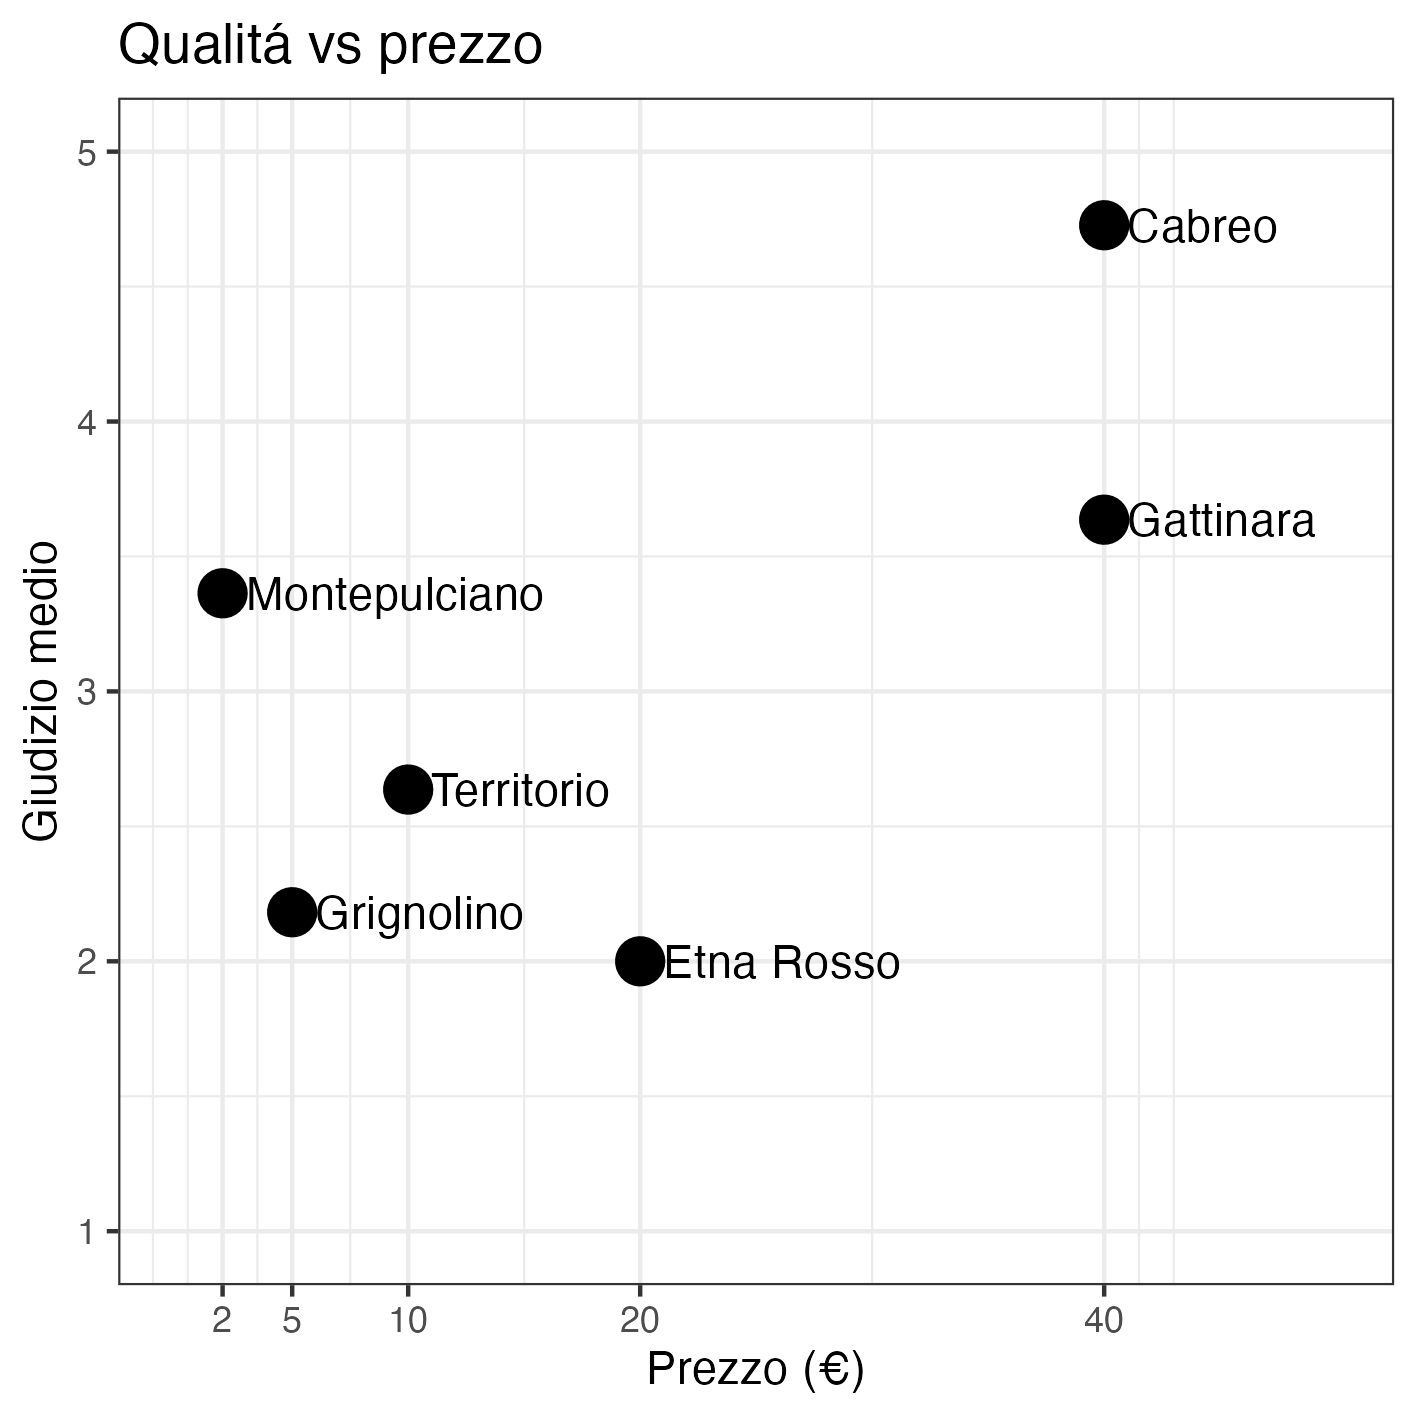
\includegraphics[width=0.5\linewidth]{plots/convenienza}

Qua il punto rosso indica il grado alcolico effettivo

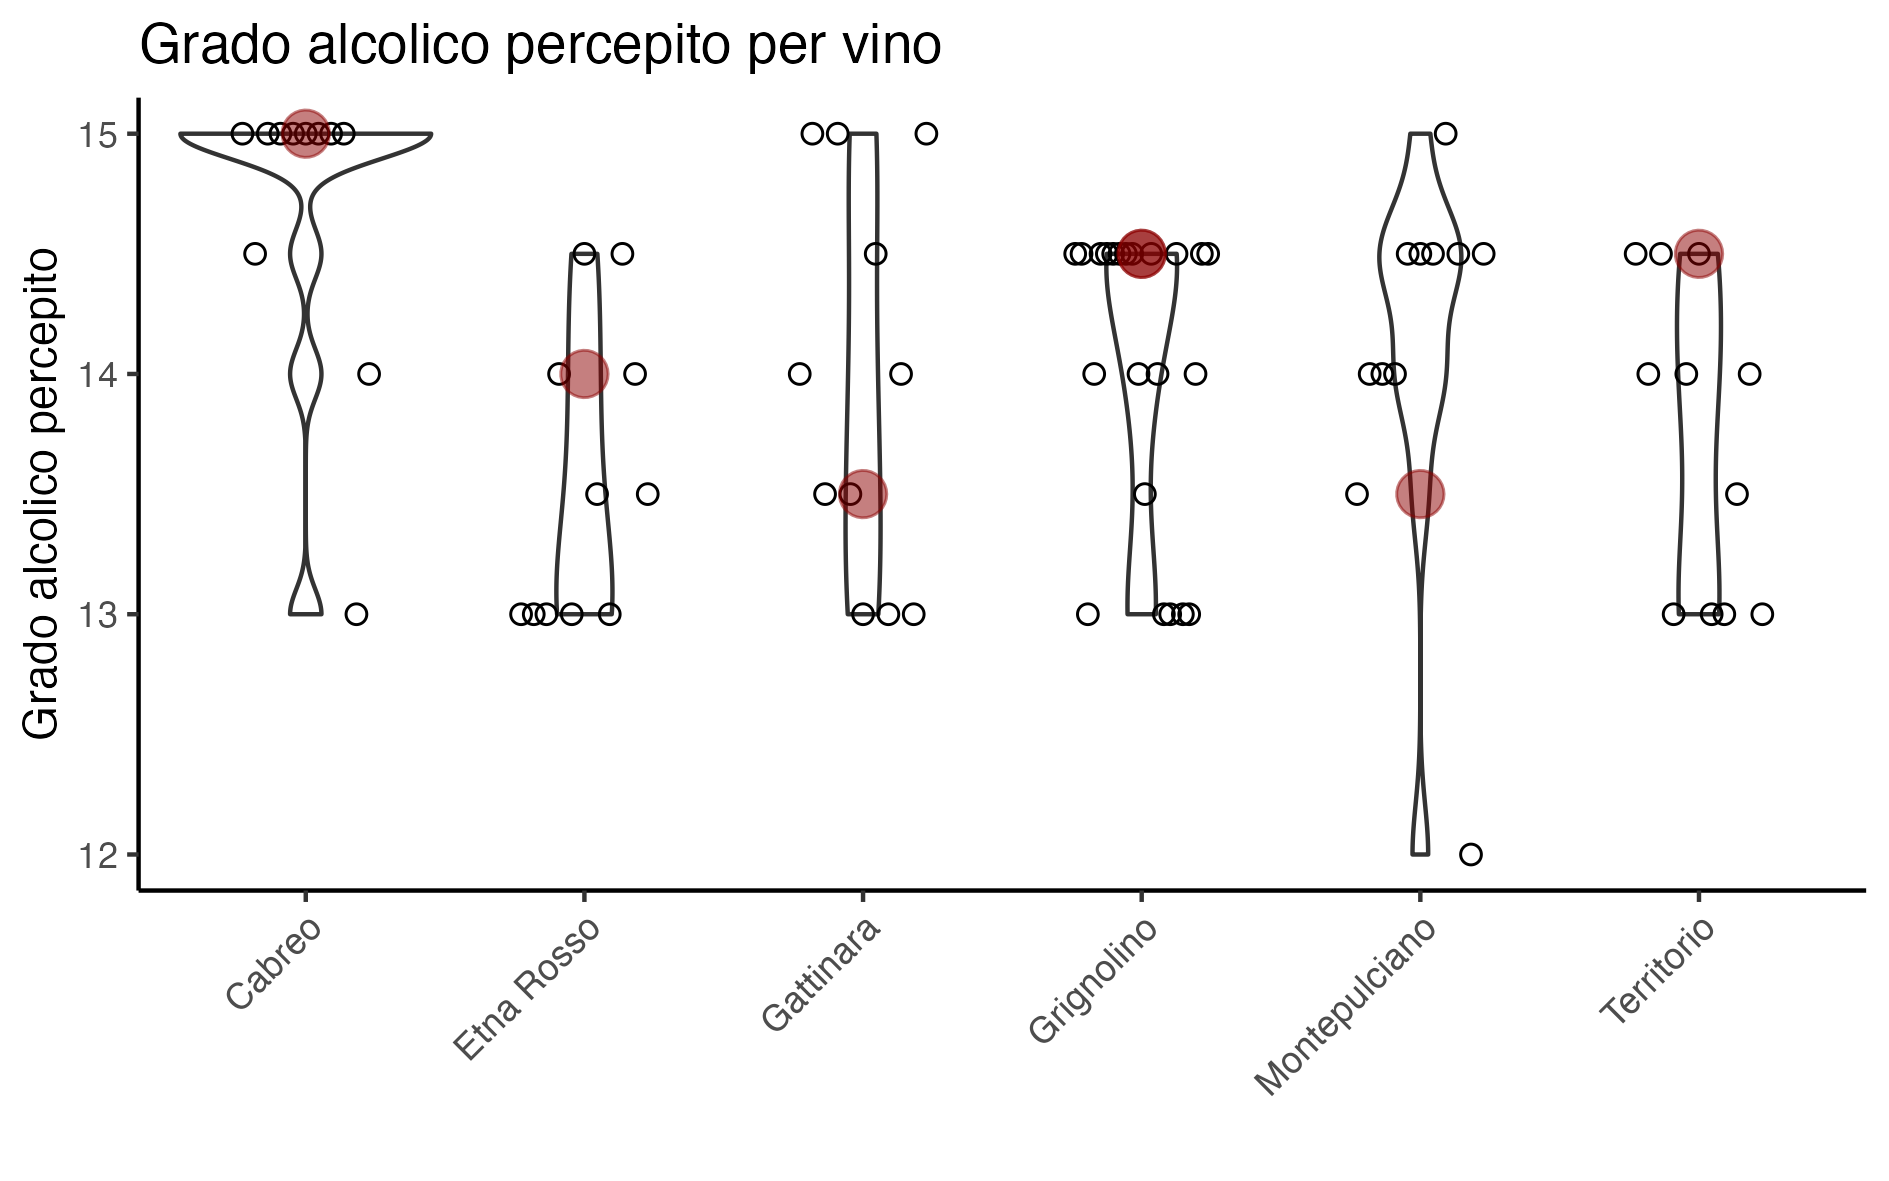
\includegraphics[width=1\linewidth]{plots/ethobywine}

\hypertarget{a-chi-piace-bere}{%
\subsection{A chi piace bere}\label{a-chi-piace-bere}}

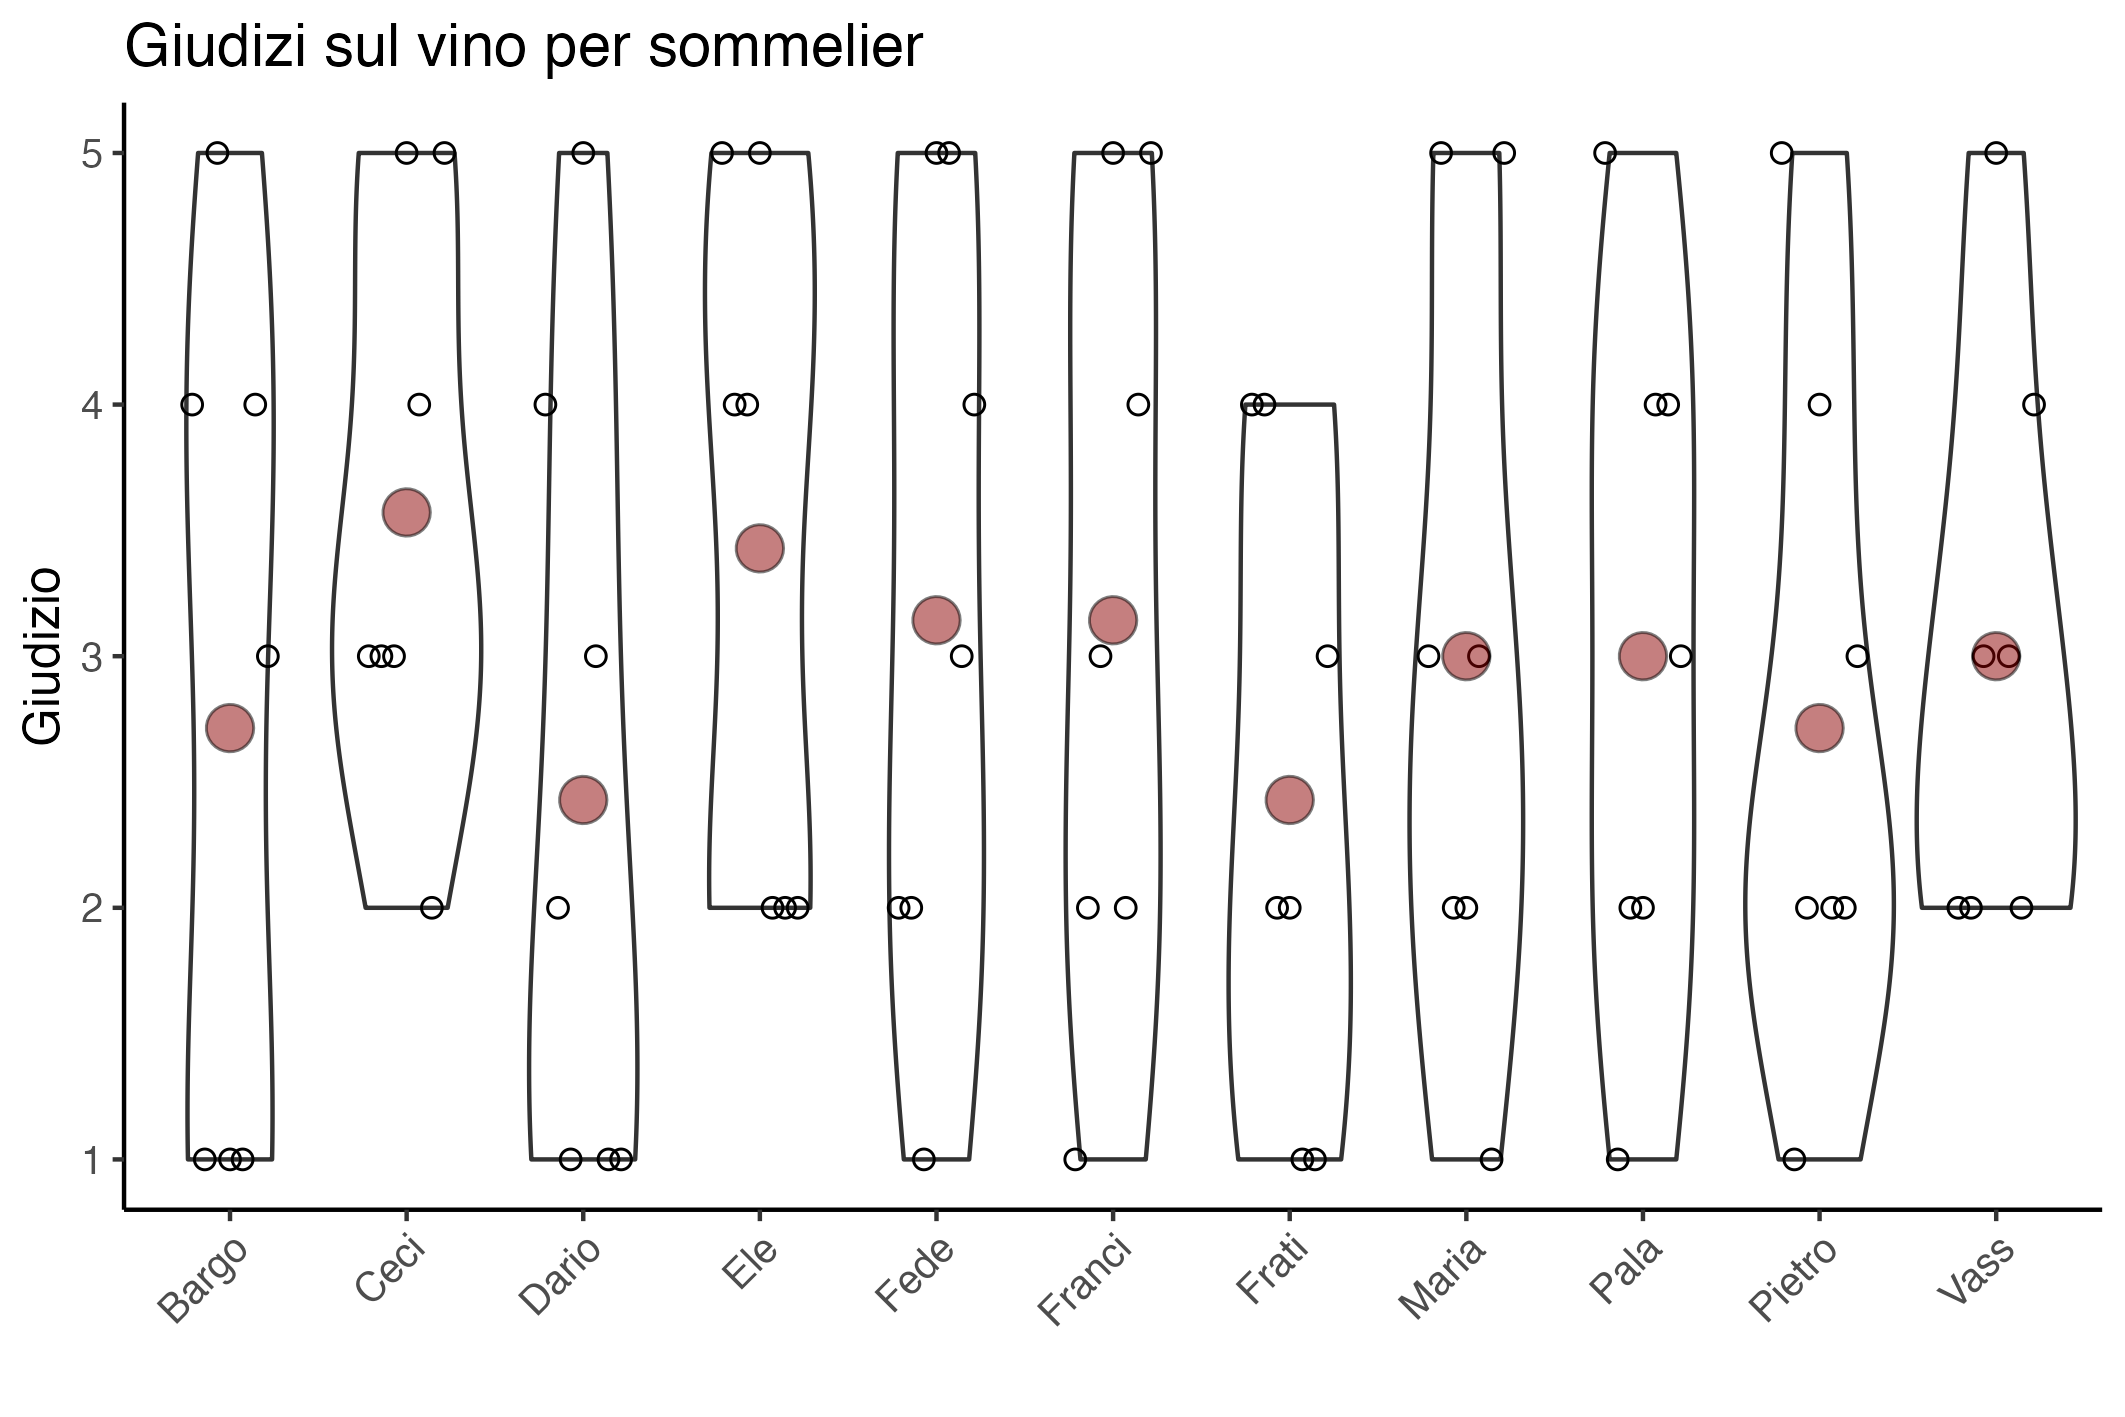
\includegraphics[width=1\linewidth]{plots/rating_per_sommelier}

\hypertarget{la-gara-dellasta}{%
\subsection{La gara dell'asta}\label{la-gara-dellasta}}

Le regole: ricevi punti uguali al costo di ciascuna bottiglie per la
quale hai offerto una cifra uguale o maggiore al suo prezzo (0 punti se
hai offerto di meno).

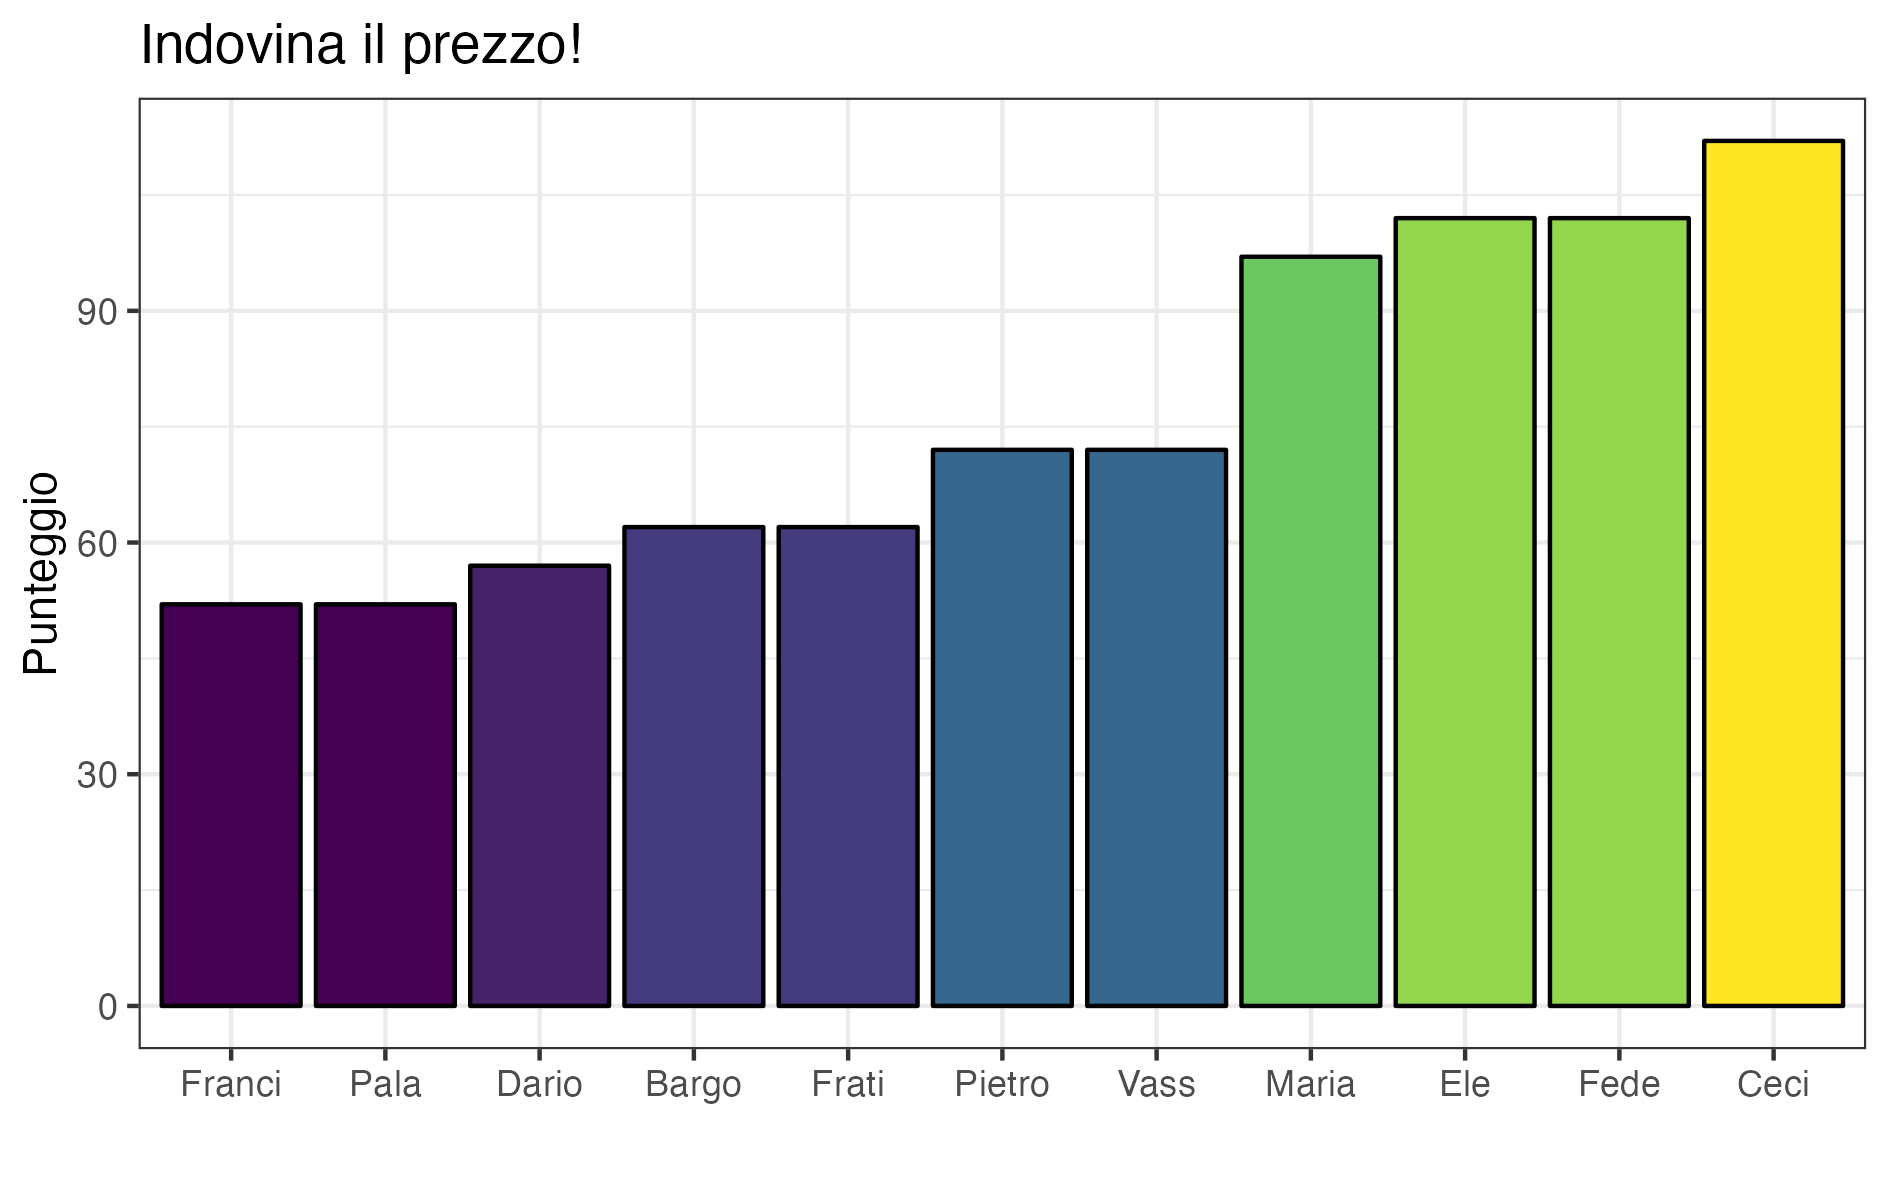
\includegraphics[width=1\linewidth]{plots/auction_rank}

\hypertarget{clustering}{%
\subsection{Clustering}\label{clustering}}

Questa é una heatmap. Il giudizio su ciascuna bottiglia é indicato dal
colore (Rosso = giudizio alto, blue = giudizio basso). Il vino giudicato
é indicato sull'asse orizzontale, e chi ha dato il giudizio sull'asse
verticale.

Gli alberelli ai lati sono due dendogrammi che indicano la `similaritá'
tra vini e tra persone che emerge dai giudizi dati. La similaritá
(misurata dalla distanza geometrica) tra due vini (o persone) si legge
dall'altezza della linea orizzonatale che li congiunge.

Per esempio Fede e Ele sono la coppia con i gusti piú simili. Se
dovessero decidere di andare a bere insieme e invitare una tersa
persona, inviterebbero Maria, che ha i gusti piu simili a loro.

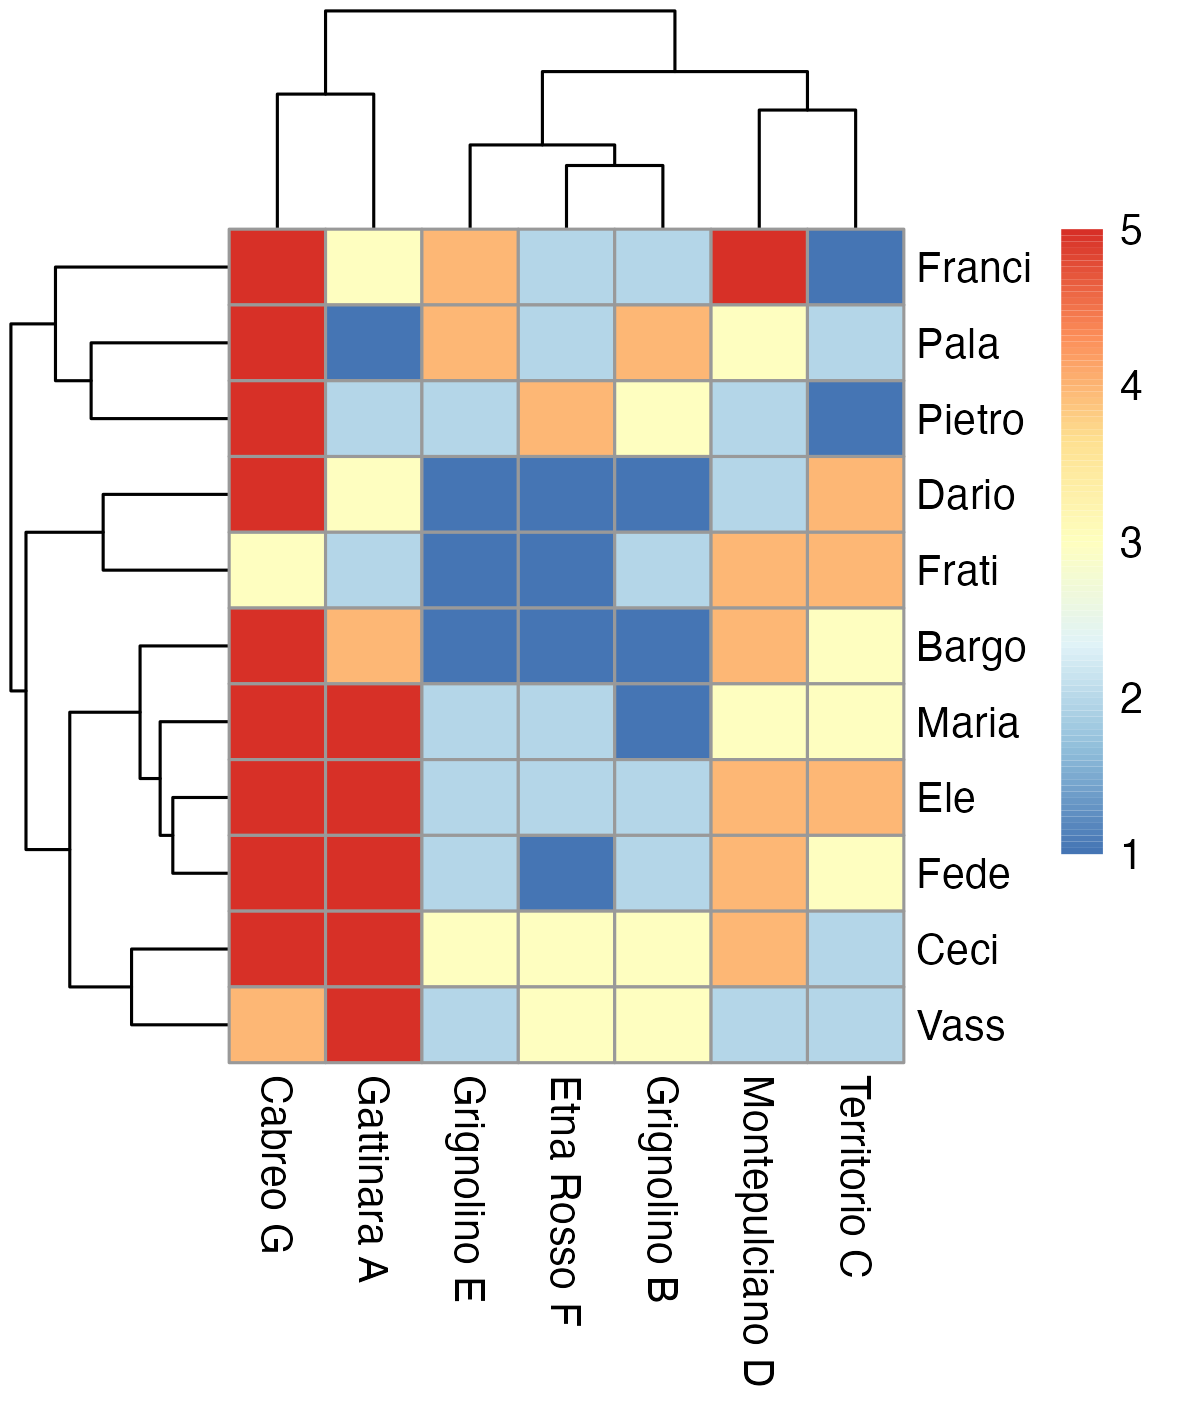
\includegraphics[width=1\linewidth]{plots/heatmap}

\end{document}
